\section{Methodology}
\subsection{Overall Research Framework}
\label{sec:overall_framework}

Our workflow integrates thermal sensation modeling with building simulation in a unified co‐simulation loop (Figure~\ref{fig:workflow}) based on Sinergym virtual testbed \cite{campoy2025sinergym}. First, at each 15-minute timestep, Sinergym queries EnergyPlus for current zone states (air temperature, humidity, etc.) and weather inputs. Second, a chosen comfort predictor—PMV, LightGBM, or PINN-VAE—estimates zone‐level thermal sensation votes (TSVs). Third, the control module computes new heating ($T_{h}$) and cooling ($T_{c}$) setpoints based on the predicted TSV (or a $\Delta T$ grid search around an interior reset). Finally, these setpoints are sent back to EnergyPlus via Sinergym’s actuator API, and the simulation advances. This cycle repeats for all timesteps across each selected climate, enabling direct comparison of energy and comfort outcomes under different control strategies.

\begin{figure}[h!]
    \centering
    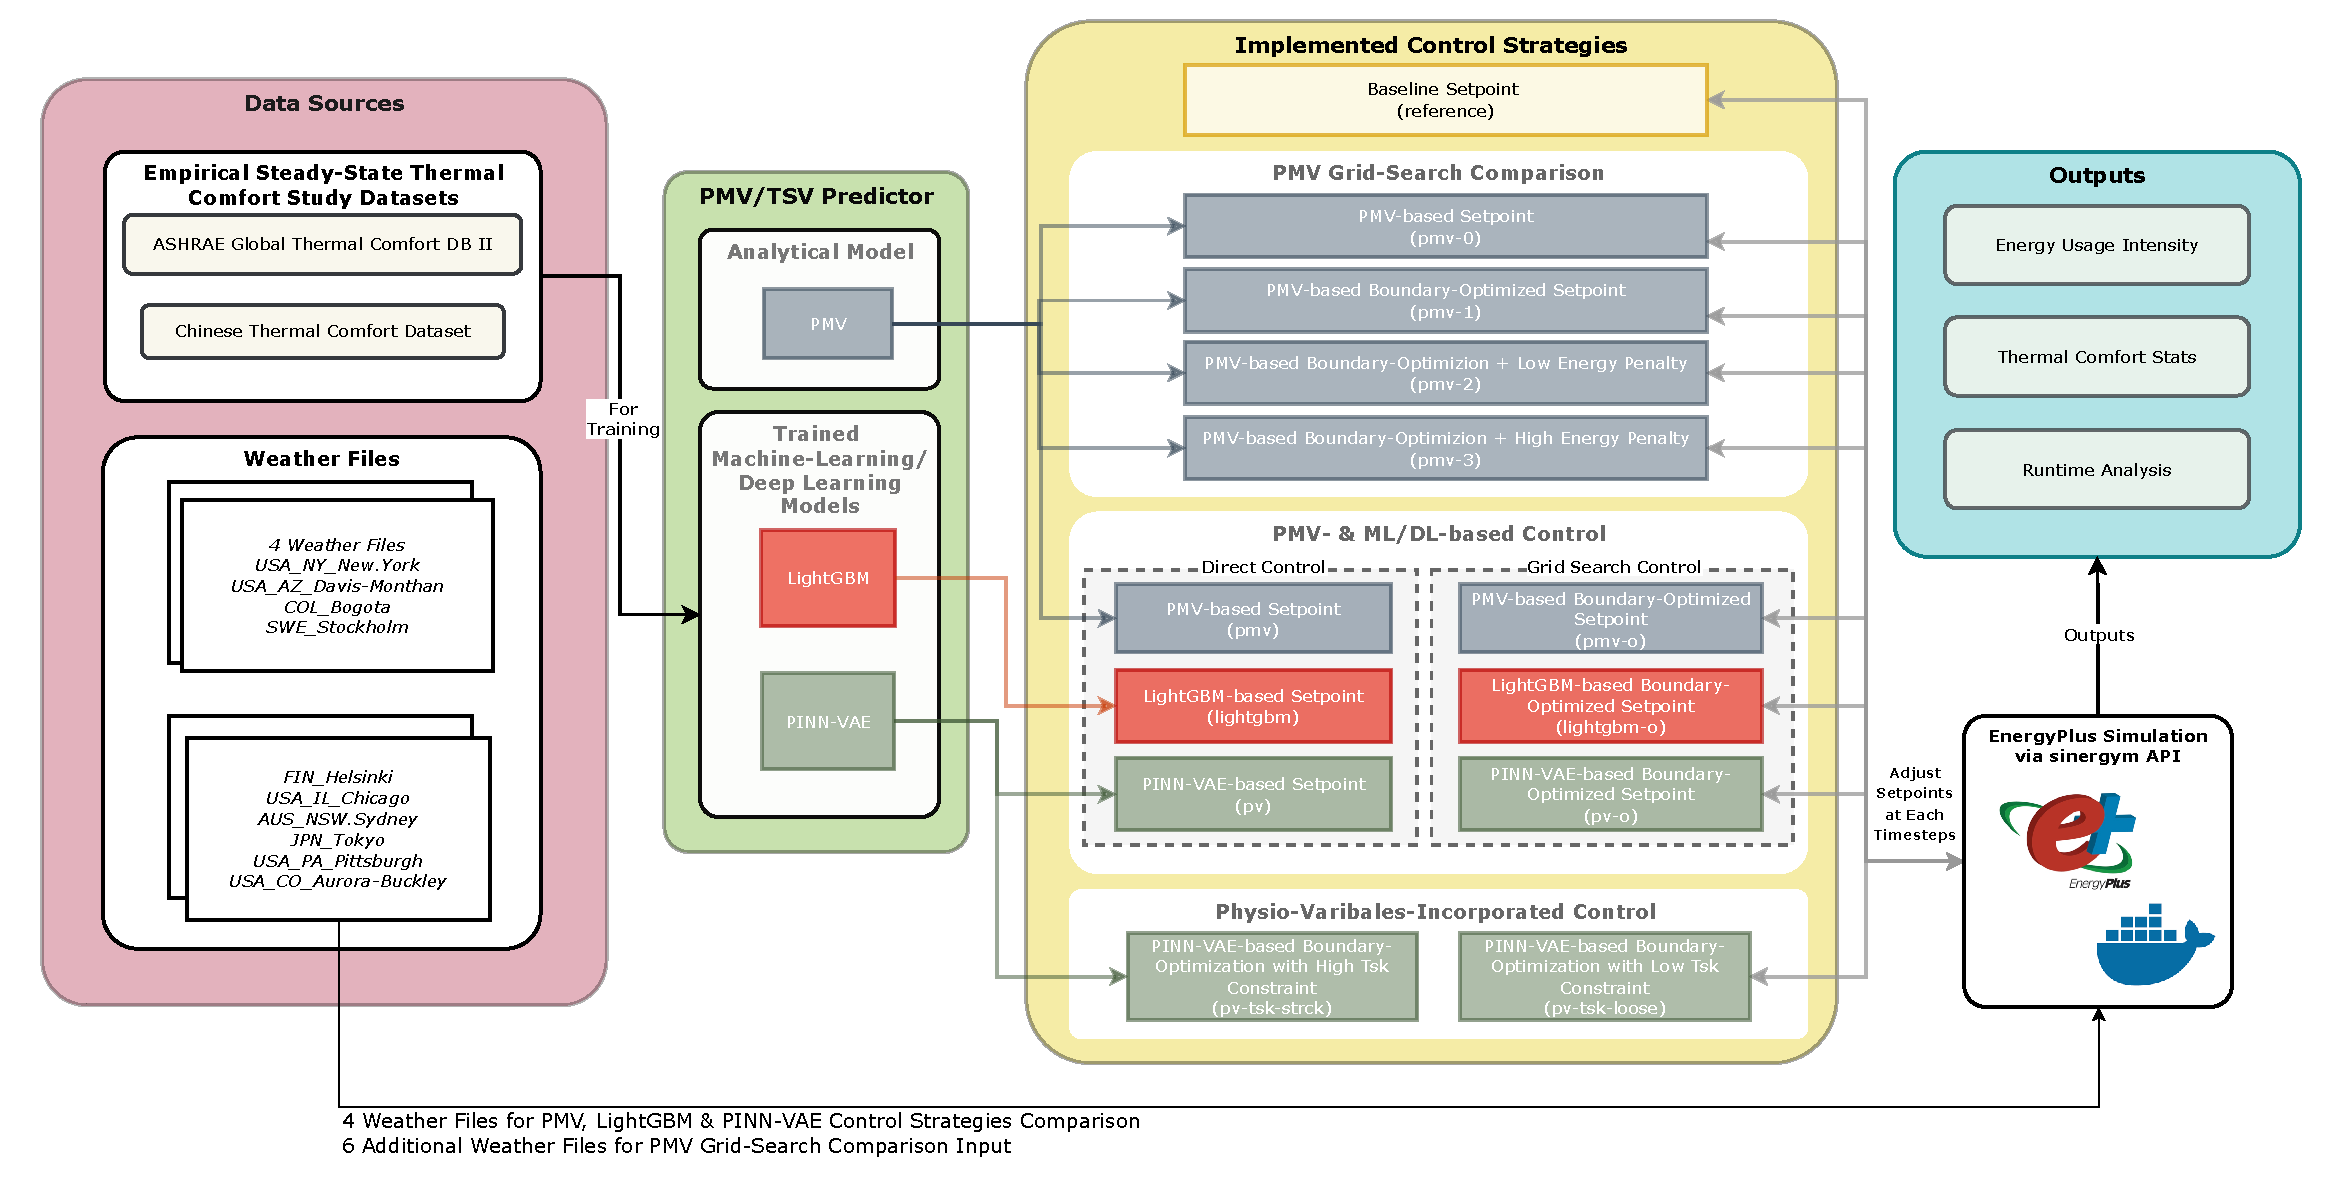
\includegraphics[width=0.95\linewidth]{figs/gridworkflow_3.pdf}
    \caption{Overall Workflow of Current Study}
    \label{fig:workflow}
\end{figure}

\subsection{Simulation Setup and Testbed Building}%Confirm we have enough on systems...?
% \subsubsection{Building Model Description and Justification}
This study adopts the \texttt{5ZoneAutoDXVAV} building model distributed with EnergyPlus \citep{energyplus}, which is commonly used for building control algorithm benchmarking \cite{gao2021deep, an2023clue, kadamala2024enhancing}. The model represents a single-story, 463 m$^2$ office building with five conditioned thermal zones and one return plenum, reflecting a prototypical open-plan office layout.

The building model supports zone-level temperature setpoint adjustment through Sinergym's actuator API, with the Energy Management System (EMS) framework enabling real-time control integration \cite{campoy2025sinergym}. We selected this model because it provides architectural symmetry and zoning simplicity that enable lightweight simulation environment and systematic algorithm testing, making it well-suited for comparative evaluation of different control strategies. While using a single building model limits generalizability to other building types and HVAC systems, this approach isolates performance differences attributable specifically to thermal comfort models and their climate interactions, rather than confounding variables from diverse building characteristics.


% \subsection{Envelope and Construction Details}
% The envelope construction is defined via abstracted \texttt{Construction} objects such as \texttt{WALL-1} and \texttt{ROOF-1}, though material layer specifications are absent in this JSON version. No window surface areas or window material properties are defined, and as such, the window-to-wall ratio (WWR) cannot be computed directly from this model. Nevertheless, the model's simplicity ensures consistent thermal response behavior and avoids geometric ambiguities \citep{drgovna2020all}.

% Each conditioned zone includes:
% \begin{itemize}
%   \item A \texttt{People} object representing occupancy density,
%   \item A \texttt{Lights} object simulating fixed lighting load, and
%   \item An \texttt{ElectricEquipment} object representing plug loads.
% \end{itemize}
% All internal gains are scheduled using \texttt{Schedule:Compact}, typically emulating business-hour profiles consistent with standard office operations. On top of that, the model includes:
% \begin{itemize}
%   \item A single \texttt{AirLoopHVAC} system with an outdoor air subsystem and return plenum (\texttt{PLENUM-1}),
%   \item Zone-level conditioning using VAV terminal units with DX cooling coils, and
%   \item Thermostat setpoint schedules that are designed to be overridden using external control via EMS actuators.
% \end{itemize}

% This setup supports cooling setpoint adjustment at the zone level, as exposed by Sinergym’s actuator API. The EMS framework facilitates real-time control from reinforcement learning agents without manual editing of EnergyPlus schedules or control logic.

% We selected this model for its:
% \begin{itemize}
%   \item \textbf{Representativeness}: Reflects the spatial and control complexity of a typical commercial office building;
%   \item \textbf{Simplicity}: Abstract geometry enables efficient simulation, particularly valuable for reinforcement learning experiments requiring thousands of rollouts;
%   \item \textbf{Modularity}: Provides a multi-zone testbed suitable for testing both centralized and decentralized control policies;
%   \item \textbf{Compatibility}: Fully integrated into the Sinergym ecosystem with predefined action and observation mappings \citep{perarnau2021sinergym};
%   \item \textbf{Reproducibility}: Used widely in prior RL-for-HVAC studies, including benchmarking efforts in \citep{gao2021deep}.
% \end{itemize}

% We understand the selection of a single IDF for this study may come with its own limitation, that the results we obtained will be specific to this building type and HVAC system. However, we believe a single, well-characterized IDF can help us isolate the performance differences that can be attributable solely to the model-enabled control strategies and their interactions with different climates, rather than variations in building systems/designs. %Reiterate this again in conclusions/discussions


\subsection{Data Source for Thermal Comfort Modeling} \label{sec:data_foundation}

As we're showing in Figure~\ref{fig:workflow}, the data source of the current study is a combination of both the ASHRAE Global Thermal Comfort Database II and the Chinese Thermal Comfort Datasets combined. This combined dataset represents a form of \textit{collective intelligence}, aggregated as 148,148 distinct pre-existing thermal sensation steady-state votes, encompassing both field and laboratory experiments from ASHRAE Thermal Comfort Database II and Chinese Thermal Comfort Datasets. This amalgamation results in a substantial corpus of 148,148 individual data points, capturing a wide diversity of environmental conditions, building typologies, geographical locations, and demographic profiles. 

The aggregation process involved careful harmonization of thermal sensation votes, typically reported on the 7-point ASHRAE scale, and standardization of input features to ensure consistency across the varied source studies. Further details on the construction, composition, and validation of this aggregated dataset can be found in [Dataset Paper Citation, if applicable, or a brief description of your harmonization process if not published separately]. This large-scale, diverse data foundation aims to foster the development of more generalized and robust thermal sensation models compared to those trained on smaller, single-source experimental data. Using this dataset, we were able to train both a machine learning (LightGBM) and deep learning (PINN-VAE, or physiological-informed neural net with variable autoencodeer) models for predicting thermal sensation are developed upon a comprehensive, aggregated dataset.

\subsection{Thermal Sensation Vote Predictors}\label{sec:comfort_models}
Aside from the analytical thermal sensation predictor of the population's mean thermal sensation, i.e. Predicted Mean Vote (PMV) \cite{Fanger1970}, we made explicit decisions on choosing the appropriate thermal sensation vote predictor. The selection process was guided by the dual objectives of robustness and innovation. We chose Light Gradient Boosting Machine (LightGBM) due to its consistently strong predictive performance with tabular datasets, as extensively validated in previous research\cite{Ke2017}. LightGBM offers computational efficiency, interpretability, and robust generalization capabilities, making it highly suitable for real-time predictive control tasks where reliability and speed are critical.

Concurrently, we introduce a novel Physics-Informed Neural Network combined with a Variational Autoencoder (PINN-VAE), specifically developed by the authors for thermal sensation prediction (publication forthcoming). This innovative model integrates physiological realism into thermal comfort modeling, explicitly leveraging Gagge's two-node model (Gagge et al., 1966) to analytically inform intermediate physiological outputs such as skin temperature ($T_{skin}$) and core body temperature ($T_{core}$). Unlike conventional predictive methods, the PINN-VAE architecture not only predicts thermal sensation with high fidelity through its deep neural network’s multi-head capability but simultaneously generates robust physiological data, significantly enhancing its utility in physiology-informed indoor environmental controls. This combination of predictive accuracy and physiological realism positions PINN-VAE as a potential transformative approach in building thermal environment management.

\subsubsection{Analytical Baseline: Predicted Mean Vote (PMV)}
\label{sec:pmv_model}
The Predicted Mean Vote (PMV) model, as developed by Fanger and standardized in ISO 7730 \citeplaceholder{ISO7730} and ASHRAE Standard 55 \citeplaceholder{ASHRAE55}, serves as an analytical baseline. PMV predicts the mean thermal sensation vote of a large group of people based on six key parameters: air temperature ($T_a$), mean radiant temperature ($T_r$), relative humidity ($RH$), air velocity ($v_{air}$), metabolic rate (Met), and clothing insulation ($I_{cl}$). In this study, when PMV-based control is active, these input parameters are derived from EnergyPlus outputs as observation of the environmental variables, coupled with predefined assumptions for occupant metabolic rate and clothing insulation, with more details documented in Section \ref{sec:control_strategies}.

We adopted standardized assumptions for occupant metabolic rates and clothing insulation based on established industry guidelines and widely accepted thermal comfort research. Specifically, a metabolic rate (MET) of 1.1 (sedentary office work) was used uniformly across simulations, consistent with recommendations by ASHRAE Standard 55\cite{ASHRAE2020}. Clothing insulation values (clo) were set to 0.65 during summer and 1.0 in winter, reflecting typical seasonal clothing variations commonly observed in office environments \cite{ASHRAE2020}.

These standardized assumptions facilitate reproducibility and enable direct comparability with established comfort models, such as PMV, while simultaneously aligning with typical office conditions documented in thermal comfort literature. Although using fixed values simplifies simulation procedures, we acknowledge potential limitations arising from the natural variability of individual occupant behavior and adaptive clothing choices in real-world scenarios.

\subsubsection{Machine Learning Benchmark: LightGBM}\label{sec:lightgbm_model}
A Light Gradient Boosting Machine (LightGBM) model is utilized as a high-performance machine learning benchmark for thermal sensation prediction. LightGBM is a tree-based gradient boosting framework known for its efficiency and accuracy \citeplaceholder{LightGBM\_Paper}. The model is trained on the aggregated dataset described in Section \ref{sec:data_foundation} to predict Thermal Sensation Vote (TSV) on the 7-point ASHRAE scale. Inputs to the LightGBM model include key environmental parameters such as [$T_a, T_r, RH, v_{air}$, clo, MET, gender, height, weight, etc.]. The model was trained using k-fold cross-validation, with hyperparameters optimized for predictive accuracy (details of training and validation are beyond the scope of this section but can be found in Appendix).

\subsubsection{Deep Learning Model: Physics-Informed Neural Network - Variational Autoencoder (PINN-VAE)}
\label{sec:pinn_vae_model}
The core novel model investigated in this study is a Physics-Informed Neural Network combined with a Variational Autoencoder (PINN-VAE), designed specifically for thermal sensation prediction and co-simulation of key physiological variables. This model architecture, detailed in a pending publication at BAE (will cite when publication is finalized), aims to overcome limitations of purely data-driven approaches by integrating domain knowledge such as physiological constraints on skin/core temperature, heat balance whilst improving the quality of input data that are missing.

In particular, the VAE component learns a robust latent representation of the input data, beneficial for handling the complexities and potential imperfections inherent in large-scale aggregated datasets. The PINN component incorporates physiological realism by embedding constraints derived from principles of human thermoregulation [e.g., based on a simplified Gagge's 2-node model \citeplaceholder{Gagge1966} or similar -- specify principles used, e.g., heat balance equations for core and skin compartments]. These physics-informed constraints guide the model to produce physiologically plausible predictions for mean skin temperature ($T_{skin}$) and core body temperature ($T_{core}$), alongside the primary output of TSV.

Inputs to the PINN-VAE are similar to the LightGBM model: [$T_a, T_r, RH, v_{air}$]. Its outputs for this study are the predicted TSV (on the 7-point ASHRAE scale), predicted $T_{skin}$, and predicted $T_{core}$. The key advantages of this PINN-VAE approach include its potential for improved generalization due to the physics-based regularization, enhanced interpretability through the prediction of intermediate physiological states, and the unique ability to leverage $T_{skin}$ as part of advanced control strategies. Training and validation details are provided in the aforementioned paper.

\section{Control Framework Implementation and Testing}
To demonstrate our co-simulation methodology's capabilities and assess its effectiveness, we implement seven distinct control strategies spanning analytical models to sophisticated deep learning approaches. This implementation serves multiple purposes: (1) confirming the framework successfully accommodates diverse model types and control logics, (2) testing the robustness of the actuator saturation handling and stochastic weather integration, and (3) generating initial insights into the relative performance of different comfort modeling approaches when deployed in actual control loops.

We emphasize that this section presents a systematic testing of our methodology rather than validation against measured building data—such empirical validation represents important future work once the framework's capabilities are established.

Our testing protocol comprises three complementary investigations:
\begin{itemize}
    \item PMV Grid-Search Optimization Study (Section 5.2): We first examine whether systematic optimization can enhance classical PMV control performance. Using 10 diverse climate locations, we compare naive PMV control against three grid-search variants to establish the potential of optimization for analytical models.
    \item Comprehensive Control Strategy Comparison (Section 5.3): We then apply our complete framework to compare seven control strategies—including both optimized and non-optimized variants of PMV, LightGBM, and PINN-VAE models—across four representative DOE climate zones. This investigation tests the framework's ability to fairly evaluate fundamentally different modeling approaches.
    \item Physiological Variable Integration (Section 5.4): Finally, we demonstrate the framework's extensibility by incorporating PINN-VAE's unique physiological predictions (skin temperature) into control logic, showcasing how our methodology enables novel control strategies beyond traditional comfort metrics.
\end{itemize}

\subsection{Control Strategies Tested}
\label{sec:control_strategies}
Across all three investigations, control strategies share common implementation characteristics. Despite their different internal logic, all controls implement a bang–bang adjustment of the heating and cooling set-points to be directly comparable against one another, with a maximum step of 1$^\circ$C per timestep (every 15 minutes). All modes share the following pre-processing steps:

\begin{itemize}
  \item \textbf{Occupancy check:} The space is considered unoccupied if it is a weekend day or outside the hours of 06:00–22:00. In unoccupied periods, the allowable comfort range is relaxed by \(\pm\SI{2}{\degreeCelsius}\).
  \item \textbf{Seasonal set‐points:} Two baseline comfort ranges, \(\left[T_\mathrm{low}^\mathrm{sum},T_\mathrm{high}^\mathrm{sum}\right]\) for summer (June 1–September 30) and \(\left[T_\mathrm{low}^\mathrm{win},T_\mathrm{high}^\mathrm{win}\right]\) for the remainder of the year, are defined a priori.  
  \item \textbf{Environmental inputs:} At each timestep, the current air temperature \(T_a\), relative humidity RH, and mean radiant temperature \(T_r\) are read from the observation vector.  
\end{itemize}

\subsubsection{Baseline Control (reference)}
\label{sec:reference_control}
The reference controller adjusts set-points based solely on the air temperature relative to the comfort range. Let
\[
(T_\mathrm{low},\,T_\mathrm{high}) = 
\begin{cases}
(T_\mathrm{low}^\mathrm{sum},\,T_\mathrm{high}^\mathrm{sum}), & \text{summer},\\
(T_\mathrm{low}^\mathrm{win},\,T_\mathrm{high}^\mathrm{win}), & \text{winter},
\end{cases}
\]
expanded by \(\pm2\)\,$\degree$C if unoccupied. Denote the current heating and cooling set‐points by \(T_\mathrm{htg}\) and \(T_\mathrm{clg}\). Then:
\begin{equation}
\begin{aligned}
\text{if } T_a &< T_\mathrm{low}: & T_\mathrm{htg}&\leftarrow T_\mathrm{htg}+1,\quad T_\mathrm{clg}\leftarrow T_\mathrm{clg}+1,\\
\text{if } T_a &> T_\mathrm{high}: & T_\mathrm{htg}&\leftarrow T_\mathrm{htg}-1,\quad T_\mathrm{clg}\leftarrow T_\mathrm{clg}-1,\\
\text{otherwise:} & & T_\mathrm{htg},\,T_\mathrm{clg}&\text{ unchanged.}
\end{aligned}
\end{equation}

\subsubsection{PMV-Based Setpoint Control (pmv)}
\label{sec:pmv_control}
The PMV controller uses the predicted Predicted Mean Vote (PMV) from the \texttt{pmv\_ppd\_iso} function, computed over the current conditioned air state. We define
\[
\mathrm{PMV} = f_\mathrm{ISO}\bigl(T_a,\,T_r,\,\mathrm{RH},\,\mathrm{met}=1.1,\,\mathrm{clo}\bigr),
\]
where \(\mathrm{clo}=0.65\) in summer and \(1.0\) in winter (adjusted for unoccupied periods as above). Denoting the mean PMV by \(\overline{\mathrm{PMV}}\), the set-point adjustment is
\begin{equation}
\begin{aligned}
\text{if } \overline{\mathrm{PMV}} &< -0.5: & T_\mathrm{htg}&\leftarrow T_\mathrm{htg}+1,\quad T_\mathrm{clg}\leftarrow T_\mathrm{clg}+1,\\
\text{if } \overline{\mathrm{PMV}} &> +0.5: & T_\mathrm{htg}&\leftarrow T_\mathrm{htg}-1,\quad T_\mathrm{clg}\leftarrow T_\mathrm{clg}-1,\\
\quad \quad & \text{otherwise:} & & T_\mathrm{htg},\,T_\mathrm{clg} \text{ unchanged.}
\end{aligned}
\end{equation}

Both controllers’ outputs \((T_\mathrm{htg},\,T_\mathrm{clg})\) are clipped to the environment’s allowable action space before being sent to EnergyPlus. These two modes serve as benchmarks against which we compare our ML­-enhanced and grid-search optimized strategies.

\subsubsection{LightGBM- and PINN-VAE- Based Control (lightgbm \& pv)}
\label{sec:lightgbm_control}

The two ML/DL-based controllers use our pre‐trained Gradient Boosting model (lightgbm) and PINN-VAE model (pv) respectively to predict the proxy occupants’ Thermal Sensation Vote (TSV) and applies a simple bang–bang adjustment of the HVAC set‐points. At each timestep, the following procedure is executed:

\begin{enumerate}
  \item \textbf{Feature assembly.} Construct a feature vector (or matrix) \(\mathbf{x}\) containing the current indoor air temperature \(T_a\), relative humidity RH, mean radiant temperature \(T_r\), clothing insulation (\(\mathrm{clo}\)), etc., exactly as in Section~\ref{sec:control_strategies}.
  \item \textbf{TSV prediction.}  
    \[
      \widetilde{\mathrm{TSV}} = \mathrm{ModelWrapper.predict}(\mathbf{x}),
    \]
    where \(\widetilde{\mathrm{TSV}}\in\mathbb{R}^n\) (one prediction per zone or sample).  
  \item \textbf{Aggregate comfort metric.} Compute the median sensation vote:
    \[
      \mathrm{TSV}_{\mathrm{med}} = \mathrm{median}\bigl(\widetilde{\mathrm{TSV}}\bigr).
    \]
  \item \textbf{Bang–bang set‐point update.} Let \(T_{\mathrm{htg}}\) and \(T_{\mathrm{clg}}\) be the current heating and cooling set‐points. Then
    \[
    \begin{cases}
      T_{\mathrm{htg}} \leftarrow T_{\mathrm{htg}} + 1,\quad
      T_{\mathrm{clg}} \leftarrow T_{\mathrm{clg}} + 1, 
      & \text{if } \mathrm{TSV}_{\mathrm{med}} < -0.5,\\[6pt]
      T_{\mathrm{htg}} \leftarrow T_{\mathrm{htg}} - 1,\quad
      T_{\mathrm{clg}} \leftarrow T_{\mathrm{clg}} - 1, 
      & \text{if } \mathrm{TSV}_{\mathrm{med}} > +0.5,\\[6pt]
      \text{unchanged,} & \text{otherwise.}
    \end{cases}
    \]
  \item \textbf{Clipping.} Finally, clip \((T_{\mathrm{htg}},T_{\mathrm{clg}})\) to the environment’s allowable action‐space.
\end{enumerate}

\noindent\emph{Computational considerations:}  
Because the wrapper instantiates a LightGBM model and meta‐information only once per episode (caching column order, category mappings, etc.), the per‐timestep cost is dominated by a single vectorized predict call, \(\mathcal{O}(n)\) in the number of samples. Memory overhead is negligible for typical zone counts (\(n<10\)).


\subsubsection{Boundary-Optimized Control (pmv-o, lightgbm-o \& pv-o)}
\label{sec:opt_boundary_pseudocode}

All boundary modes perform the same grid-search over a set of temperature offsets \(\Delta T\) to drive the predicted comfort metric as close as possible to the comfort boundaries \(\pm0.5\). The PMV or TSV values are predicted with different prediction models, i.e., PMV, LightGBM and PINN-VAE (abbreviated hereinafter as pmv-o, lightgbm-0 and pv-o). We summarize the procedure in Algorithm~\ref{alg:boundary_opt}.

\begin{algorithm}[ht]
\caption{Boundary‐Optimized Set‐Point Adjustment}\label{alg:boundary_opt}
\KwIn{Current features $\mathbf{x}$, set‐points $(T_\text{htg},T_\text{clg})$, predictor $\mathsf{pred}(\cdot)$}
\KwData{Shifts $\mathcal{D}=\{-2,\dots,2\}$}
Build batch $\mathbf{X}\leftarrow[\mathbf{x}+\delta_1;\dots;\mathbf{x}+\delta_m]$\;
$\mathbf{y}\leftarrow\mathsf{pred}(\mathbf{X})$\;
Reshape into $\mathbf{Y}\in\mathbb{R}^{m\times n}$\;
\For{$i\leftarrow1$ \KwTo $m$}{
  $s_i^-\leftarrow|\mathrm{med}(\mathbf{Y}_i)+0.5|$\;
  $s_i^+\leftarrow|\mathrm{med}(\mathbf{Y}_i)-0.5|$\;
}
$\delta^-\leftarrow\arg\min_i s_i^-$; $\delta^+\leftarrow\arg\min_i s_i^+$\;
$\delta^*\leftarrow\arg\min_{\delta\in\{\delta^-,\delta^+\}}|\delta|$\;
$T_\text{htg}\mathbin{+{\mkern-8mu}=}\delta^*$; $T_\text{clg}\mathbin{+{\mkern-8mu}=}\delta^*$\;
Clip to action space\;
\end{algorithm}

Because we reset any extreme setpoints to (19$^\circ$C, 27$^\circ$C) before evaluating ∆T, none of the candidate shifts (\pm2$^\circ$C, \pm1$^\circ$C, \pm0.5$^\circ$C) ever crosses the hard bounds [12$^\circ$C, 23.25$^\circ$C]×[23.25$^\circ$C, 30$^\circ$C], thereby eliminating actuator saturation in the grid-search process.
\noindent\emph{Practical considerations:}  
The single batch predict call reduces overhead compared to looping over shifts. Total complexity remains \(\mathcal{O}(mn)\) model evaluations, with memory to hold \(m\!n\) feature rows. In our experiments (\(m=9,n<10\)), this executes in under 150\,ms per timestep, making it suitable for real‐time or near‐real‐time HVAC control loops.

\subsubsection{Physiological Variables Incorporated Boundary-Optimized Control (pv-tsk-strick \& pv-tsk-loose)}
\label{sec:pv_tsk_control}
The PINN-VAE model, with its intrinsically physiological-constrained model design, is capable of predicting physiological variables, including skin temperature ($T_{skin}$), apart from TSV value. Built upon the aforementioned boundary-optimized PINN-VAE control strategy (\texttt{pv-o}), we further incorporate the predicted $T_{skin}$ into control strategy to better leverage the capacities of the advanced model. Specifically, at each action point, the agent evaluates whether both the predicted TSV and $T_{skin}$ falls within the target range while maintaining the same grid search strategy to find the minimum setpoint deviation that meet the both criterion (\texttt{pv-tsk-strict}). Alternatively, as a more relaxed control strategy, the comfort requirement is considered to be met if either the TSV or $T_{skin}$ falls within its respective comfort range (\texttt{pv-tsk-loose}). The $T_{skin}$ target range is set at a conservative comfort range $32.8\,^\circ\mathrm{C} \leq T_{skin} \leq 33.8\,^\circ\mathrm{C}$ as reported by Weiwei et al. \cite{liuUseMeanSkin2015}. Since pv-o itself never generates clipped setpoints, these pv-tsk variants likewise avoid any actuator saturation.

\subsection{Inputs and Outputs}
\paragraph{Weather Files used}\label{sec:weather_noise}
We employed twelve EPW-format weather files as the nominal dataset for year-long EnergyPlus simulations\footnote{Typical EPW fields and structure are defined in the EnergyPlus Weather File Data Dictionary\cite{EPW_Data_Dictionary}}.  
From these, four representative files—selected according to DOE climate zone classifications (e.g., 2B: hot‐dry; 4A: mixed‐humid; 5C: cool‐marine; 7: cold)—were used to benchmark the control strategies outlined in Section~\ref{sec:control_strategies}.  

An additional eight EPW files were reserved for extended validation of PMV-based set‐point optimization. To account for meteorological variability and reinforce the robustness of our findings, we enabled the stochastic weather module in the Sinergym package, which injects Gaussian perturbations (zero mean, $\sigma$ = 2.5 $\degree$C) into the dry-bulb and radiant temperature series for each timestep\cite{Sinergym_Stochastic}.


This stochastic weather module is critical for establishing the statistical robustness of our findings. Rather than evaluating control performance under a single deterministic weather year—which could lead to overfitting to specific weather patterns—each simulation experiences unique weather realizations. The Gaussian perturbations ($\sigma$ = 2.5°C) applied to dry-bulb and radiant temperatures at every timestep ensure that our control strategies are tested against a distribution of possible weather conditions, not just historical averages. This approach inherently provides statistical validation by demonstrating that the performance rankings and energy savings remain consistent despite weather variability, strengthening confidence in the generalizability of our results.
\begin{itemize}
  \item \textbf{EPW format:} Comma-delimited with hourly records for 8,760 hours, containing standard fields such as Year, Month, Day, Hour, Dry-Bulb Temperature, and Sky Infrared Radiation\cite{EPW_Format}.
  \item \textbf{Climate selection:} Four climates (2B, 4A, 5C, 7) chosen to span hot-dry, mixed-humid, cool-marine, and cold conditions.
  \item \textbf{Stochastic noise:} Gaussian noise ($\mu$=0, $\sigma$=2.5 $\degree$C) added to temperature fields via Sinergym’s stochastic environments\cite{Sinergym_Stochastic}, enhancing sensitivity analysis and result stability.
\end{itemize}

\paragraph{Performance Metrics (Overview)}
To compare the different control strategies (reference, PMV, LightGBM, PINN-VAE and optimized variants), we will evaluate the outputs from the EnergyPlus simulation across:  
\begin{itemize}
  \item Annual energy consumption by end use types (and percent savings relative to the reference), on top of energy usage intensitivies.  
  \item Fraction of occupied hours with TSV within the $\pm$0.5 comfort/thermal neutral band.  
  \item Average simulation runtime per annual run.  
\end{itemize}
The results of the comparison of these metrics across different runs are reported in the results section of this paper and further discussed in corresponding discussion sections.%Add more?
The precise mathematical definitions and any additional robustness or combined‐FoM (Combined Figure of Merit) metrics are given in Section~\ref{sec:performance_metrics}.%? I guess perhaps add some more to appendix?


\subsection{Actuator Limits and Saturation Considerations}
\label{sec:actuator_saturation_method}

In \texttt{5ZoneAutoDXVAV} example file, the default heating and cooling setpoints are hard‐limited beyond the EnergyPlus allowable range to
\[
12\,^\circ\mathrm{C} \;\leq T_{h} \;\leq 23.25\,^\circ\mathrm{C} 
\quad\text{and}\quad
23.25\,^\circ\mathrm{C} \;\leq T_{c} \;\leq 30\,^\circ\mathrm{C}.
\]
Whenever a controller requests a setpoint outside these bounds, Sinergym automatically clips it to the nearest limit—a phenomenon we refer to as \emph{actuator saturation}. If left unaddressed, any logic that naively drives $T_{h}<12\,^\circ\mathrm{C}$ or $T_{c}>30\,^\circ\mathrm{C}$ will simply “stick” at the boundary, masking the true comfort–energy trade‐off.

In our initial “pure” implementations (PMV inversion, LightGBM inversion, PV inversion), we observed that repeated attempts to push setpoints beyond $12\,^\circ\mathrm{C}$ or $30\,^\circ\mathrm{C}$ yielded clipped controls that never returned to an interior value. To mitigate this, we introduced a boundary‐optimized grid‐search protocol as follows:  
\begin{enumerate}
  \item \textbf{Interior Reset.} Whenever the previous setpoint pair $(T_{h},T_{c})$ falls outside $[13\,^\circ\mathrm{C},29\,^\circ\mathrm{C}]$, we immediately reset to $(19\,^\circ\mathrm{C},\,27\,^\circ\mathrm{C})$.  
  \item \textbf{$\Delta T$ Grid Search.} From that interior point, we evaluate seven candidate offsets
    \[
      \Delta T \;\in\; \{-2.0,\,-1.0,\,-0.5,\,0.0,\,+0.5,\,+1.0,\,+2.0\}\,\text{°C}
    \]
    simultaneously. Because $(19\,^\circ\mathrm{C} \pm 2\,^\circ\mathrm{C})$ and $(27\,^\circ\mathrm{C} \pm 2\,^\circ\mathrm{C})$ lie strictly within the allowable $[12\,^\circ\mathrm{C},\,30\,^\circ\mathrm{C}]$ band, none of these candidates are ever clipped.  
  \item \textbf{Final Gap Enforcement.} After selecting the best $\Delta T$ (based on $\bigl|\lvert \text{comfort}\rvert - 0.5\bigr|$ plus an energy penalty), we reimpose a $2\,^\circ\mathrm{C}$ heating–cooling gap and then perform one last clamp to guarantee feasibility.  
\end{enumerate}

By acknowledging Sinergym’s actuator saturation up front and embedding this reset + $\Delta T$ grid logic in the methodology, we ensure that none of our “optimized” setpoints are artifactual products of clipping. This approach eliminates “sticking” at $12\,^\circ\mathrm{C}$ or $30\,^\circ\mathrm{C}$ and preserves a meaningful comfort gradient throughout the simulation.